\documentclass[final]{beamer}
\usepackage[utf8]{inputenc}
\usepackage[T1]{fontenc}
\usepackage{lmodern}
\usepackage{booktabs}
\usepackage{listings}
\definecolor{colString}{rgb}{0.6,0.1,0.1} 
\definecolor{Green}{rgb}{0.1,0.5,0.1}



%%%%%%%%%%%%%%%%
%%% LISTINGS %%%
%%%%%%%%%%%%%%%%
\lstset{%configuration de listings 
	float=hbp,% 
	language={C},%
	morekeywords={},%
	basicstyle=\ttfamily\protect\fontsize{16pt}{16pt}\protect\selectfont, % 
	backgroundcolor=\color{white},%
	identifierstyle=\color{black}, % 
	keywordstyle=\color{blue}, % 
	stringstyle=\color{colString}, % 
	commentstyle=\color{Green}, % 
	columns=flexible, % 
	keepspaces=true,  % keeps spaces in text, useful for keeping indentation of code
	escapeinside={\%*}{*)},%
	tabsize=4, % 
	frame=l, % 
	frameround=tttt, % 
	extendedchars=true, % 
	showspaces=false, % 
	showstringspaces=false, % 
	%numbers=left, % 
	numbersep=5pt,
numberstyle=\protect\fontsize{16pt}{16pt}\protect\selectfont\ttfamily\color{black}, % 
	breaklines=true, % 
	xleftmargin=20pt, %
	breakautoindent=true, % 
	captionpos=b,% 
} 

\mode<presentation> { 
\usetheme{SERTIF}
}
%\usecolortheme{Entrepreneur}
%\usecolortheme{ComingClean}
%\usecolortheme{ConspiciousCreep}
\usepackage[orientation=portrait,size=a0,scale=1.4]{beamerposter}
\usepackage{tcolorbox}
\tcbset{%
    noparskip,
    colback=white, %background color of the box
    colframe=normalTitleBlockColor, %color of frame and title background
    coltext=black, %color of body text
    coltitle=black, %color of title text 
    %fonttitle=\bfseries,
    %valign upper=center,
    %boxsep=2mm,
    boxrule=1.5mm,
    alerted/.style={coltitle=red, 
                     colframe=gray!40},
    example/.style={coltitle=black, 
                     colframe=green!20,             
                     colback=green!5},
    }

\title[]{
Evaluation of the Embedded Software Robustness\\ Against Intentional Fault
Injections by Simulation
}

\author[
]{
    Maël Berthier\inst{2},
    Cécile Dumas\inst{1},
    Louis Dureuil\inst{1,3},
    Thanh-Ha Le\inst{2},
    Marie-Laure Potet\inst{3},
    Lionel Rivière\inst{2}
}

\institute{
    \inst{1} CEA-LETI \\
    \inst{2} SAFRAN MORPHO \\
    \inst{3} VERIMAG, University of Grenoble
}

\beamertemplatenavigationsymbolsempty
\begin{document}

 \begin{frame}[fragile]{} 
    \vfill
    \begin{tcolorbox}[adjusted title={\centering \Large SERTIF project}]
    \begin{columns}
    \begin{column}{0.49\linewidth}
    \begin{itemize}
    \item Evaluate software implementations against fault injection attacks targeting data and control flow.
    \item Propose robustness evaluation criteria of software implementations.
    \item Compare the simulation tools independently developed by the partners.
    \item Build a benchmark of smartcard applications directed towards fault injection.
    \end{itemize}
    \end{column}
    \begin{column}{0.48\linewidth}
    \centering
    \includegraphics[width=0.80\textwidth]{img/schemaPoster}
    \end{column}
    \end{columns}
    \end{tcolorbox}

    \vfill
	\vspace{0.5cm}
    \begin{tcolorbox}[adjusted title={\centering \Large Fault simulators}]

    \begin{columns}[t]
    \begin{column}{0.31\linewidth}
    \begin{tcolorbox}[
    colback=white, %background color of the box
    colframe=normalTitleBlockColor, %color of frame and title background
    colframe=gray!20, %color of frame and title background
    boxrule=1mm,
    coltext=black, %color of body text
    coltitle=black, %color of title text
    bottom=2mm,
    equal height group=A,
    valign = center,
    adjusted title={\large Lazart \normalsize (by VERIMAG)}]
\begin{itemize}
\item C code robustness evaluation against fault injection using symbolic
execution.
	\vspace{1cm}
    \begin{columns}
    \begin{column}{0.40\textwidth}
    \centering 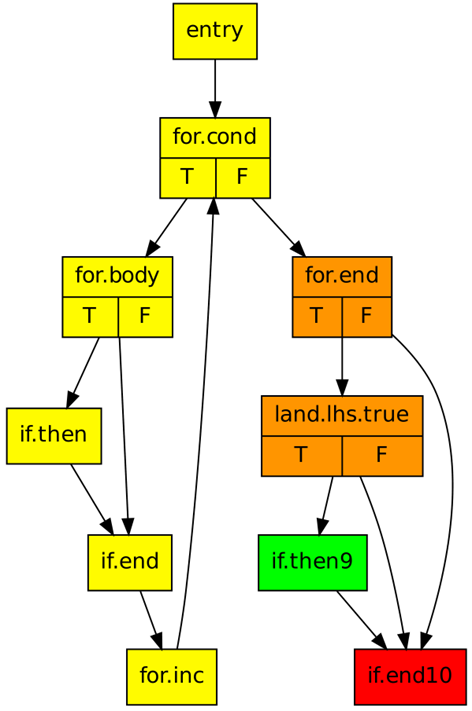
\includegraphics{img/colored_cfg}
    \end{column}
    \begin{column}{0.60\textwidth}
    \centering \includegraphics[width=0.95\textwidth]{img/LazartFramework}
    \end{column}
    \end{columns}
	\vspace{1cm}
    
\item Goal: Reach or avoid a CFG block.
	\vspace{3mm}
\item Fault model: control-flow condition inversion.
	\vspace{3mm}
\item Based on Klee, a concolic tool for LLVM.
	\vspace{3mm}
\item A complete diagnostic: activates all possible paths and fault injections.
	\vspace{3mm}
\item Scales to multiple fault injection scenarios.
\end{itemize}
    \end{tcolorbox}
    \end{column}
    \begin{column}{0.31\linewidth}
    \begin{tcolorbox}[
    colback=white, %background color of the box
    colframe=normalTitleBlockColor, %color of frame and title background
    colframe=gray!20, %color of frame and title background
    coltext=black, %color of body text
    coltitle=black, %color of title text 
    bottom=2mm,
    boxrule=1mm,
    equal height group=A,
    adjusted title={\large EFS \normalsize (by MORPHO)}]

\begin{itemize}
\item \textbf{E}mbedded \textbf{F}ault \textbf{S}imulator: embedded into the
target device (smartcard, micro-controller), at the low-level assembly code.
\item Fault mechanism: a self-test program with a high priority level, granting
access to critical registers, memories and execution flow of the smartcard.
\item Fault models: code alterations (instruction skipping, instruction
alteration), data modification at register level.
\item Advantages: 
\begin{itemize}
       \item fault injections on physical component.
       \item side-channel observations.
       \end{itemize}
       \end{itemize}
       \centering \includegraphics[width=0.95\textwidth]{img/EFSFramework}
    \end{tcolorbox}
    \end{column}
    \begin{column}{0.31\linewidth}
    \begin{tcolorbox}[
    colback=white, %background color of the box
    %colframe=normalTitleBlockColor, %color of frame and title background
    colframe=gray!20, %color of frame and title background
    coltext=black, %color of body text
    coltitle=black, %color of title text 
    equal height group=A,
    boxrule=1mm,
    valign = center,
    adjusted title={\large CELTIC \normalsize (by CEA-LETI)}]
    \begin{itemize}
\item Native smartcard binaries simulation with fault injection.
	\vspace{4mm}
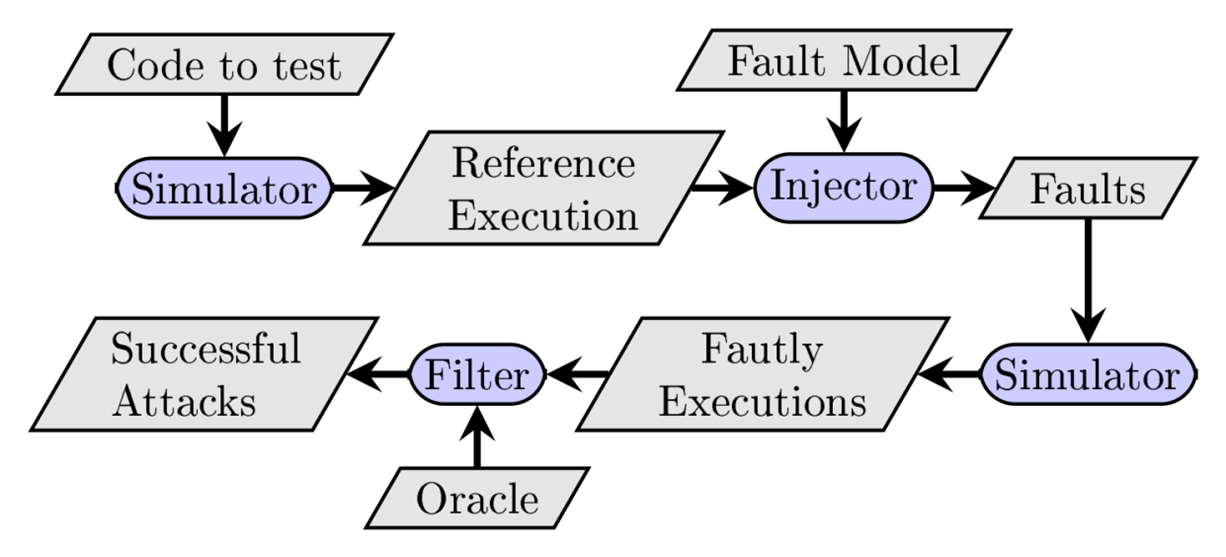
\includegraphics{img/celtic_workflow}
\item Custom Domain Specific Language to decode and execute native instructions.
\item Fault model: volatile memory perturbation, can model data and code faults.
\item User-defined victory oracles.
	\vspace{4mm}
    \end{itemize}
    \begin{columns}
    \begin{column}{0.50\linewidth}
	    \centering 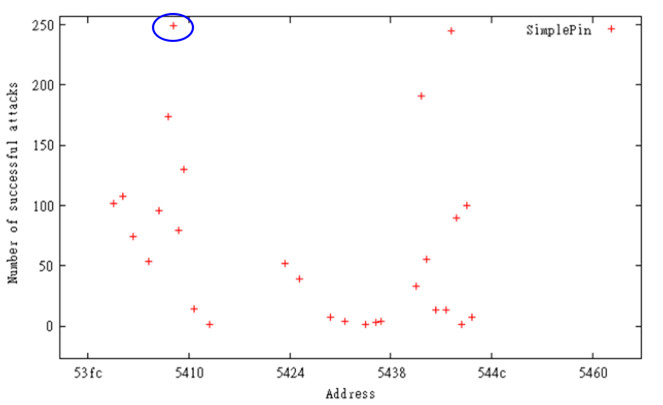
\includegraphics[width=0.99\textwidth]{img/celtic_output}
    \end{column}
    \begin{column}{0.50\linewidth}
	    \centering 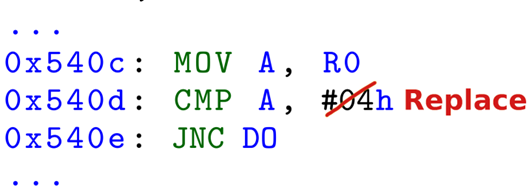
\includegraphics[width=0.99\textwidth]{img/code_excerpt}
    \end{column}
    \end{columns}
    \end{tcolorbox}
    \end{column}
    \end{columns}
    \end{tcolorbox}

    \vfill
    \vspace{-1cm}
    \begin{columns}[t]
      \begin{column}{.49\textwidth}
        \begin{tcolorbox}[adjusted title={\centering \Large Combining high-level and
        low-level simulations}]
        {\em \tiny(Paper “Combining High-Level and Low-Level Approaches to Evaluate
Software Implementations Robustness Against Multiple Fault Injection Attacks”,
FPS 2014)}

%%%%%%%%%%%%%%%%%%%%%%%%%%%%ù

        \begin{itemize}
        
\item {{\bf Observation:} vulnerability sets detected by Lazart and EFS often intersect,
however each simulator also detects vulnerabilities that are not revealed by
the others tool.}
        \end{itemize}

	{\bf\footnotesize Example {\em byteArrayCompare}}
	\vspace{-1cm}
\begin{columns}[T]
\begin{column}{.48\linewidth}
%\begin{figure}
%\centering \includegraphics[width=0.99\textwidth]{img/byteArrayCompare.pdf}
\begin{lstlisting}[name={byteArrayCompare},
basicstyle=\ttfamily\protect\fontsize{19pt}{19pt}\protect\selectfont, % 
                   label=lst:byteArrayCompare,
                   numbers=left]
// Byte array comparison
static byte byteArrayCompare(byte* a1, byte* a2){
  int i       = 0;
  byte status  = BOOL_FALSE;
  byte diff    = BOOL_FALSE;
  for (i=0; i<pinSize; i++)
      if (a1[i] != a2[i])
              diff = BOOL_TRUE;
  if ((i == pinSize) && (diff == BOOL_FALSE))
      status = BOOL_TRUE;
  return status;
}
\end{lstlisting}

%\end{figure}
\end{column}
\begin{column}{.48\linewidth}
    \vspace{-13mm}
	\begin{table}
		\small
		\centering
		\begin{tabular}{p{0.20\linewidth}cc@{\hspace{1cm}}p{0.30\linewidth}c}
			\multicolumn{2}{c}{Lazart} && \multicolumn{2}{c}{EFS} \\
			\cmidrule{1-2}\cmidrule{4-5} 
			\centering \em Fault number & \em Attacks &&
			\centering \em Skipped instructions & \em Attacks \\
			\cmidrule{1-2}\cmidrule{4-5} 
			\centering 0 & 0 &&
			\centering 0 & 0 \\
			\centering 1 & 1 &&
			\centering 1 & 4 \\
			\centering 2 & 1 &&
			\centering 2 & 1 \\
			\centering 3 & 0 &&
			\centering 3 & 1 \\
			\centering 4 & 1 &&
			\centering 4+ & 0 \\
			\cmidrule{1-2}\cmidrule{4-5} 
			\centering Total & 3 &&
			\centering Total & 6 \\
			\cmidrule{1-2}\cmidrule{4-5} 
		\end{tabular}
	\end{table}

\end{column}
\end{columns}
    \vspace{8.5mm}
	{\bf\footnotesize Example {\em verifyPIN}}
	\vspace{-1cm}
\begin{columns}[T]
\begin{column}{.48\linewidth}
\begin{lstlisting}[
label=lst:verifyPINLocal, numbers=left]
equal = BOOL_TRUE; 
for(i=0 ; i<pinSize; i++) { // Main comparison
    equal = equal & ((userPin[i] != cardPin[i]) ? BOOL_FALSE : BOOL_TRUE); 
    stepCounter++; 
}
if(equal == BOOL_TRUE) { 
     if(equal != BOOL_TRUE)			   // Double test
         goto counter_measure; 		   
     ptc = MAX_TRIES; 		   // PIN Try counter (PTC) backup
     ptcTst = -MAX_TRIES; 	   // Second backup for test
     if(ptc != -ptcTst) // Verifies the new value 
         goto counter_measure;
     authenticated = 1; // Authentication status update
     if(stepCounter == INITIAL_VALUE + 4)
         return EXIT_SUCCESS; 
} else { 
     authenticated = 0; 
     if (stepCounter == INITIAL_VALUE + 4)
         goto failure; 
}	
\end{lstlisting}
%\begin{figure}
%\centering 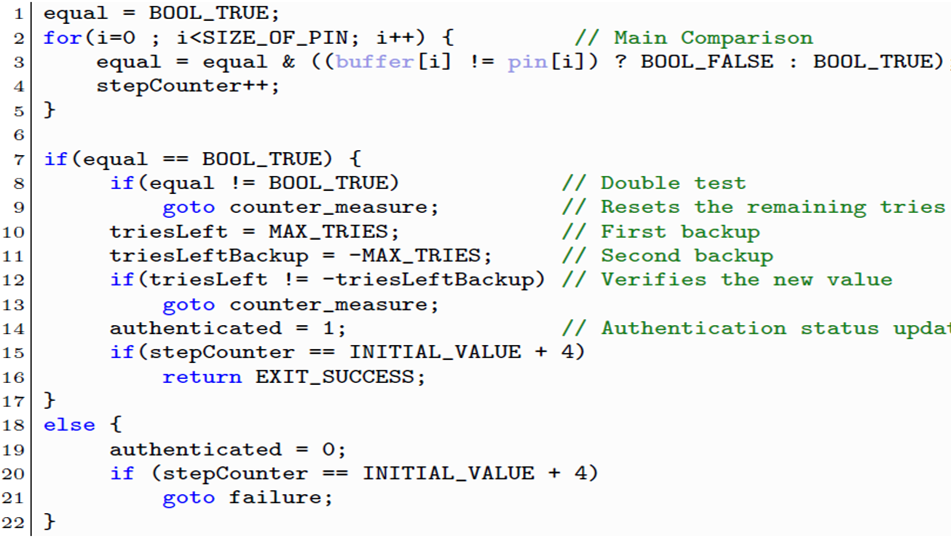
\includegraphics[width=.99\textwidth]{img/verifypin}
%\end{figure}
\end{column}
\begin{column}{.48\linewidth}
    \vspace{-13mm}
	\begin{table}
		\small
		\centering
		\begin{tabular}{p{0.20\linewidth}cc@{\hspace{1cm}}p{0.30\linewidth}c}
			\multicolumn{2}{c}{Lazart} && \multicolumn{2}{c}{EFS} \\
			\cmidrule{1-2}\cmidrule{4-5} 
			\centering \em Fault number & \em Attacks &&
			\centering \em Skipped instructions & \em Attacks \\
			\cmidrule{1-2}\cmidrule{4-5} 
			\centering 0 & 0 &&
			\centering 0 & 0 \\
			\centering 1 & 0 &&
			\centering 1 & 1 \\
			\centering 2 & 2 &&
			\centering 2 & 1 \\
			\centering 3 & 0 &&
			\centering 3 & 0 \\
			\centering 4 & 1 &&
			\centering 4 & 0 \\
			  &   &&
			\centering 5+ & 1 \\
			\cmidrule{1-2}\cmidrule{4-5} 
			\centering Total & 3 &&
			\centering Total & 3 \\
			\cmidrule{1-2}\cmidrule{4-5} 
		\end{tabular}
	\end{table}

\end{column}
\end{columns}

\begin{itemize}
\item {{\bf Optimization:} combining the simulation tools revealed enhanced vulnerability
detection, accuracy and coverage.}
\end{itemize}

\begin{columns}[T]
\begin{column}{0.48\textwidth}
\begin{table}
\footnotesize
\begin{tabular}{cccp{3.5cm}c}
	\multicolumn{5}{c}{\em byteArrayCompare} \\
\toprule
 \em Approach &  \em Tests &  \em Attacks & 
\centering \em Detection Rate &  \em Time \\
\midrule
Lazart & 56 & 27 (3) & \centering 11,7\% & $\approx$ 3s \\
EFS & 2652 & 204 (6) & \centering 2,9\% & $\approx$ 9mn \\
Both & $56+572$ & 20 (4) & \centering 20\% & $\approx$ 2mn \\
\bottomrule
\end{tabular}
\end{table}
\end{column}
\begin{column}{0.48\textwidth}
\begin{table}
\footnotesize
\begin{tabular}{cccp{3.5cm}c}
	\multicolumn{5}{c}{\em verifyPIN} \\
\toprule
\em Approach &  \em Tests &  \em Attacks & 
\centering \em Detection Rate &  \em Time \\
\midrule
Lazart & 49 & 18 (3) & \centering 16,6\% & $<$ 3s \\
EFS & 4528 & 72 (2) & \centering 2,7\% & $\approx$ 17mn \\
Both & $49+720$ & 14 (3) & \centering 21.4\% & $\approx 1.5$mn \\
\bottomrule
\end{tabular}
\end{table}
\end{column}
\end{columns}
\end{tcolorbox}

      \end{column}
      \hspace{0.3cm}
      \begin{column}{.49\textwidth}

        \begin{tcolorbox}[colframe=alertTitleBlockColor,
        %colback=alertBlockColor,
        colback=white,
        adjusted title={\centering \Large Fault simulation benchmark}]
	\textbf{Goals:}
\begin{itemize}
\item Providing a common set of representative code examples (with or without countermeasures), hardened against fault injection.
\item Testing fault simulation tools on the benchmark to:
\begin{itemize}
          \item Quantify and qualify the robustness of code examples.
          \item Establish relevant comparisons between the tools.
          \end{itemize}
\end{itemize}
\vspace{4.5mm}
\textbf{Organization:}
\begin{itemize}
\item Two categories of examples:
\begin{itemize}
          \item Code snippets to evaluate tools and their fault models.
          \item Full implementations, to qualify their relative robustness.
        \end{itemize}
\item For each code example, we provide:
\begin{itemize}
           \item Source code (in C).
           \item Victory oracle (conditions for an attack to be successful).
           \item Toolchain (OS, compiler) and compilation invocation.
           \item Relevant information about the expected memory layout.
           \end{itemize}
\end{itemize}
\vspace{5.5mm}
\centering 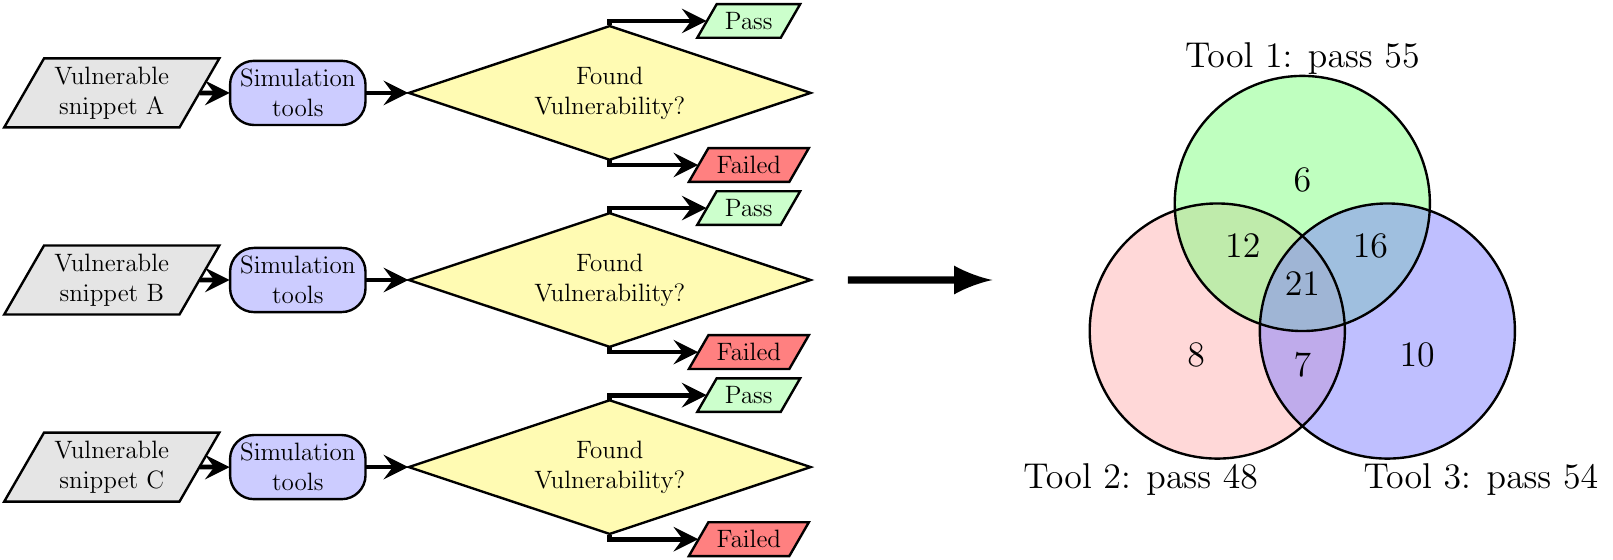
\includegraphics[width=0.99\textwidth]{img/schemaPosterBench.pdf}
        \end{tcolorbox}
\vspace{1.45cm}
        \begin{tcolorbox}[
        adjusted title={\centering \Large Perspectives of SERTIF},
        %colframe=exampleTitleBlockColor,
        colframe=exampleBlockColor,
        %colback=exampleBlockColor,
        ]
        \begin{itemize}
\item Extension to secure elements or smart secure devices.
\item Robustness against high-order fault injection.
\item Studies of compiler impact on robustness and counter-measures.
        \end{itemize}
        \end{tcolorbox}

      \end{column}
    \end{columns}
\end{frame}

\end{document}
